\documentclass[conference]{IEEEtran}
\IEEEoverridecommandlockouts
% The preceding line is only needed to identify funding in the first footnote.
% If that is unneeded, please comment it out.

\usepackage{amsmath,amssymb,amsfonts}
\usepackage{graphicx}
\usepackage{textcomp}
\usepackage{xcolor}
\usepackage{cite}
\usepackage{url}

\def\BibTeX{{\rm B\kern-.05em{\sc i\kern-.025em b}\kern-.08em
    T\kern-.1667em\lower.7ex\hbox{E}\kern-.125emX}}

\begin{document}

\title{Compressed Decoupled Z-Cache\\
{\footnotesize ECE 757 Project Report}
}

\author{\IEEEauthorblockN{Sreeraj Kannakarankodi, Noah Madison Scott, Tudor Fabian Popa,\\
Vidhyanandhan Sathish Kumar, Abhinarayani Velu Radhakrishnan}
\IEEEauthorblockA{\textit{University of Wisconsin--Madison} \\
Madison, WI, USA}
}

\maketitle

\begin{abstract}
We propose a unification of the Z-Cache and Bit-Plane Cache Compression (BPC)
systems, such that the disadvantages of Z-Cache, that are normally solved by
increasing the cache size, are addressed by the compression solution. There is
an inherent incompatibility between the standard implementation of Z-Cache and
most cache compression algorithms due to the variable block size. Thus we
propose a decoupled design that attempts to cleanly solve this incompatibility
without invoking major modifications to the Z-Cache and BPC systems. Ultimately
we find that our solution performs very well on easily compressible data, such
as during financial simulations. But in the cases of scientific or
heavy-computation benchmarks, which have low data similarity across a cache
line, the data compresses poorly, and our implementation performs worse than
baseline.
\end{abstract}

\begin{IEEEkeywords}
cache compression, Z-Cache, skewed-associative cache, bit-plane compression,
last-level cache, gem5
\end{IEEEkeywords}

\section{Introduction and Motivation}
Z-Cache virtually expands the associativity of a cache by ``hijacking'' the
ways of other addresses during a cache miss and victim selection. It selects
which lines to hijack by modifying the skewed cache design; each line is
selected by a different hash function. Z-Cache's effectiveness relies on the
fact that the probability that its virtual-way system interferes with important
cache lines is rather low~\cite{sanchez2010zcache}. The chance of this
destructive interference lowers with larger and larger caches.

It then behooves us to want to give Z-Cache as large a cache as possible to
work with. The last-level cache (LLC) is a prime candidate for this, but
doubling the LLC freely is not always possible, depending on the power or die
budget.

We then propose that the solution lies in cache compression. By applying
compression to the cache, we can emulate a larger cache with only a fraction of
the die space and power consumption. If some cache compression technique
provides a 2:1 compression ratio, then we would expect the new Z-Cache to
perform equivalent to a Z-Cache with double the cache capacity.

\section{Background and Design Challenges}
For our compression algorithm choice, we chose Bit-Plane Cache
Compression~\cite{kim2016bpc}, chosen due to its ease of implementation and
simple design. We had hoped to use a delta-style compressor, like the XOR
Cache~\cite{pan2025xorcache}, but time did not allow.

Our goal for the design was to provide something that required little to no
changes to BPC or Z-Cache. Most of the logic needed to be implemented in a
``glue'' module, rather than worked into the other components. This was to make
the design more attractive, as it would minimize the difficulty of
verification.

The first major issue that we faced was an inherent incompatibility between a
compressed cache and Z-Cache. Z-Cache performs ``cuckoo cache'' style moves
between selected possible-victim blocks, selected in a
``victim-tree''~\cite{sanchez2010zcache, pagh2004cuckoo}. This means, for any
given victim-tree constructed, all victims that will undergo this cuckoo
shuffle have to be the same size. This is a fundamental force against
compression, which will produce blocks of varying sizes depending on how
effective the compression was for that data.

To both fulfill our design goals and solve the inherent incompatibility of the
design, we had to consider decoupled designs: systems that isolated each
component from the rest of the system as much as possible, such that we can
attempt to solve these incompatibilities with deferment and abstraction.

\begin{figure*}[!t]
  \centering
  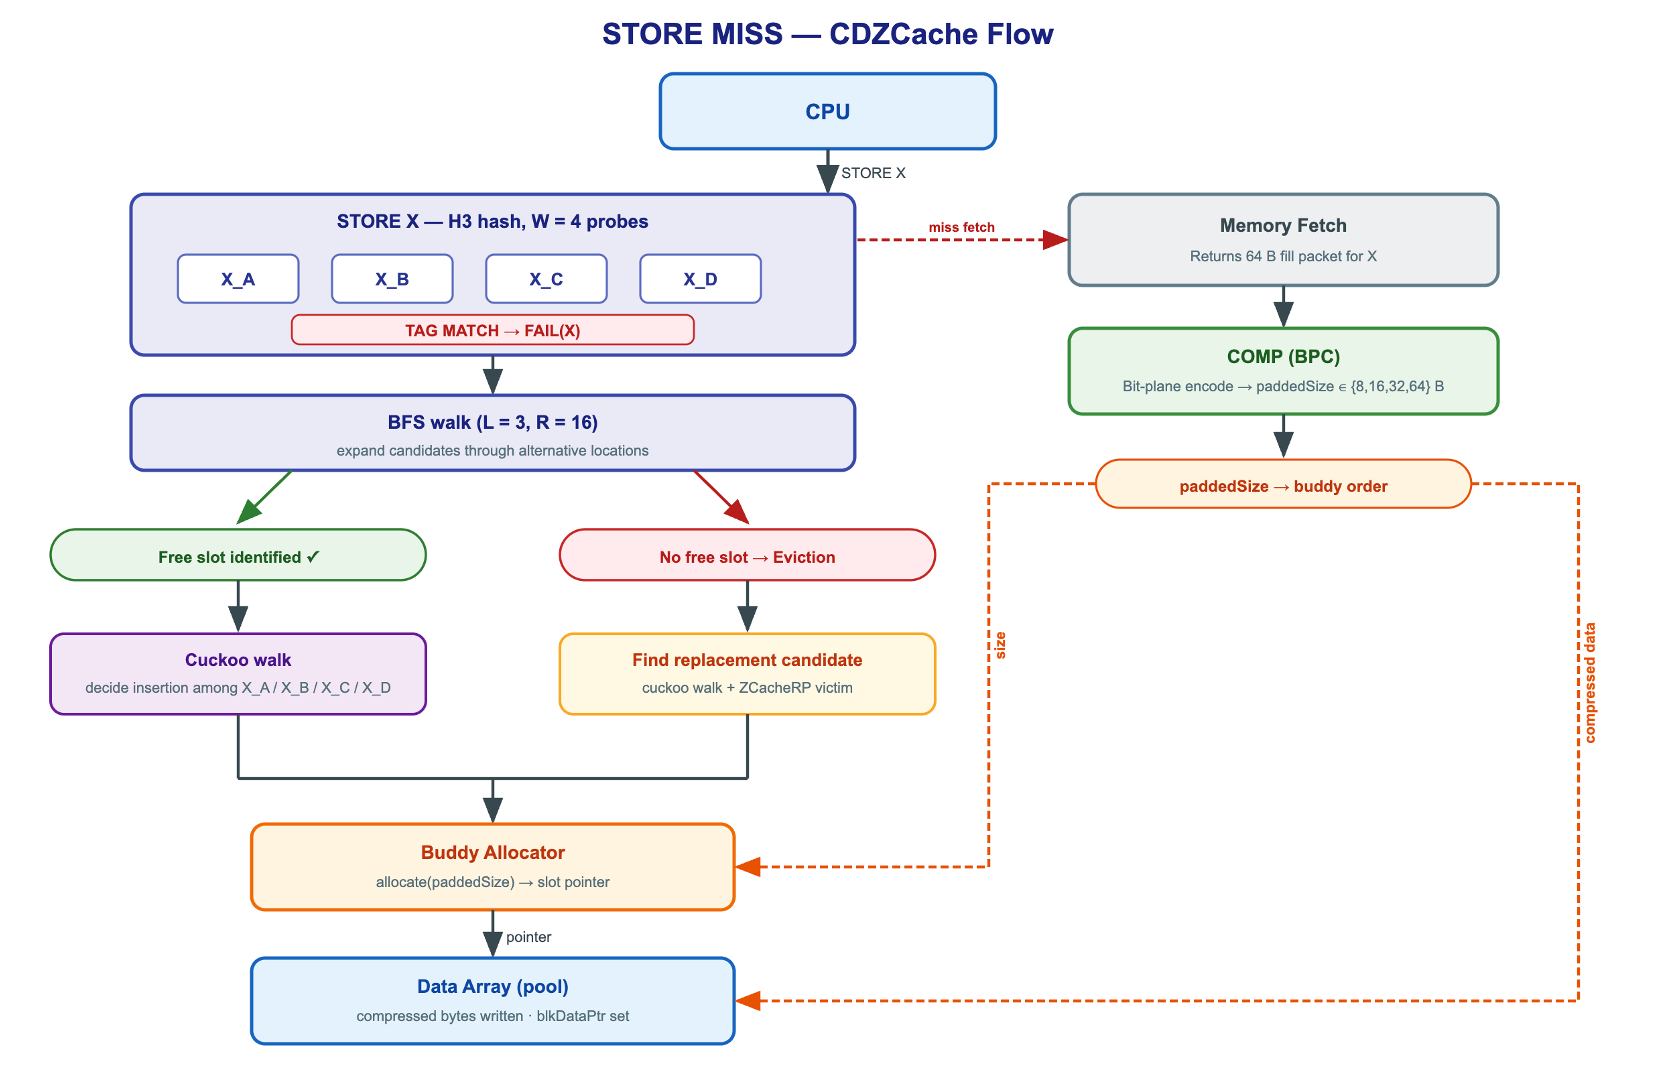
\includegraphics[width=0.85\textwidth, keepaspectratio]{cdz-diagram.png}
  \caption{High-level CDZ-Cache diagram.}
  \label{fig:arch}
\end{figure*}

\section{CDZ-Cache Design}
We propose a Compressed Decoupled Z-Cache (CDZ-Cache) system
(Fig.~\ref{fig:arch}). Our design can be split into three major parts: the
compressor system, the data allocation system, and the Z-Cache system.

\subsection{Compressor System}
The BPC compressor system has been slightly modified to restrain the variation
in block sizes it can return. It has been restricted to the sizes of 8 bytes,
16 bytes, 32 bytes, and 64 bytes. The size of the compressed block is padded to
the nearest restricted size before it is sent to the data allocation system.

\subsection{Data Allocation System}
The data allocation system is the ``glue'' that brings the BPC and Z-Cache
systems together. It is composed of two parts: a data array, and a
buddy-allocator system. Blocks are sent from the compressor to the system,
which will then allocate room for them in the data array. The resulting pointer
to the allocation is then sent to the Z-Cache. If the data array suffers
external fragmentation to the point that an allocation fails, it will trigger a
defragmentation eviction.

The chance of a buddy allocator, managing four block sizes, to experience
external fragmentation is low, but to address the corner case we implement a
pseudo-random defragmentation policy. Every couple cycles, one of four
pointers, one for each block size, will access a pseudo-random address
(generated with a linear-feedback shift register). If this address is of that
pointer's appropriate block size, the pointer will hold it forward. Once a
defragmentation event happens, the pointer of the block size needed will
trigger a ``silent'' eviction of that block and notify the Z-Cache. This
eviction is silent, as it does not invoke the Z-Cache policy logic; it is a
simple forced writeback-and-invalidate.

\subsection{Z-Cache System}
The Z-Cache system has been slightly modified to now hold the pointers returned
from the data array as its basic cache block, rather than any actual data. This
means the skewing and cuckoo policy logic can remain completely unchanged,
while still managing variable-sized blocks at a higher level. As each block is
managed by a fixed-sized pointer, this solves the incompatibility.

\section{Evaluation}
\subsection{Methodology}
We implemented CDZ-Cache as a gem5 LLC
policy~\cite{binkert2011gem5, lowepower2020gem5}. It was benchmarked on the
PARSEC 2.1 benchmark suite~\cite{bienia2008parsec, bienia2011thesis}, and
compared to a normal Z-Cache of equivalent size and one of double size as
baselines. gem5 was set to use a dual-core Timing Simple CPU with a 32\,KB L1
per-core cache, and a shared 256\,KB L2 cache, which acted as the LLC. In the
case of the second baseline, the L2 size was doubled.

\subsection{Results}
As seen in Fig.~\ref{fig:results}, our implementation performs just as well if
not better than a double-capacity Z-Cache under \textit{Swaptions} and achieves
halfway the performance of the double-capacity benchmark under
\textit{Blackscholes}. However, it was only able to match the base benchmark
under \textit{Streamcluster} and \textit{Canneal}, and it performed
significantly worse under \textit{Fluidanimate} and \textit{Freqmine}.

The effectiveness of our implementation seems to rely heavily on the
effectiveness of the BPC implementation. Our compression implementation only
helps when the application's data has numerical regularity. For the two
financial workloads (\textit{Blackscholes} and \textit{Swaptions}) there is a
clear advantage. For simulation and data-mining workloads with diverse or
irregular data, BPC performs very poorly, and the compression and decoupling
system only seem to hold the performance of standard Z-Cache back, rather than
enhance it.

\begin{figure*}[!t]
  \centering
  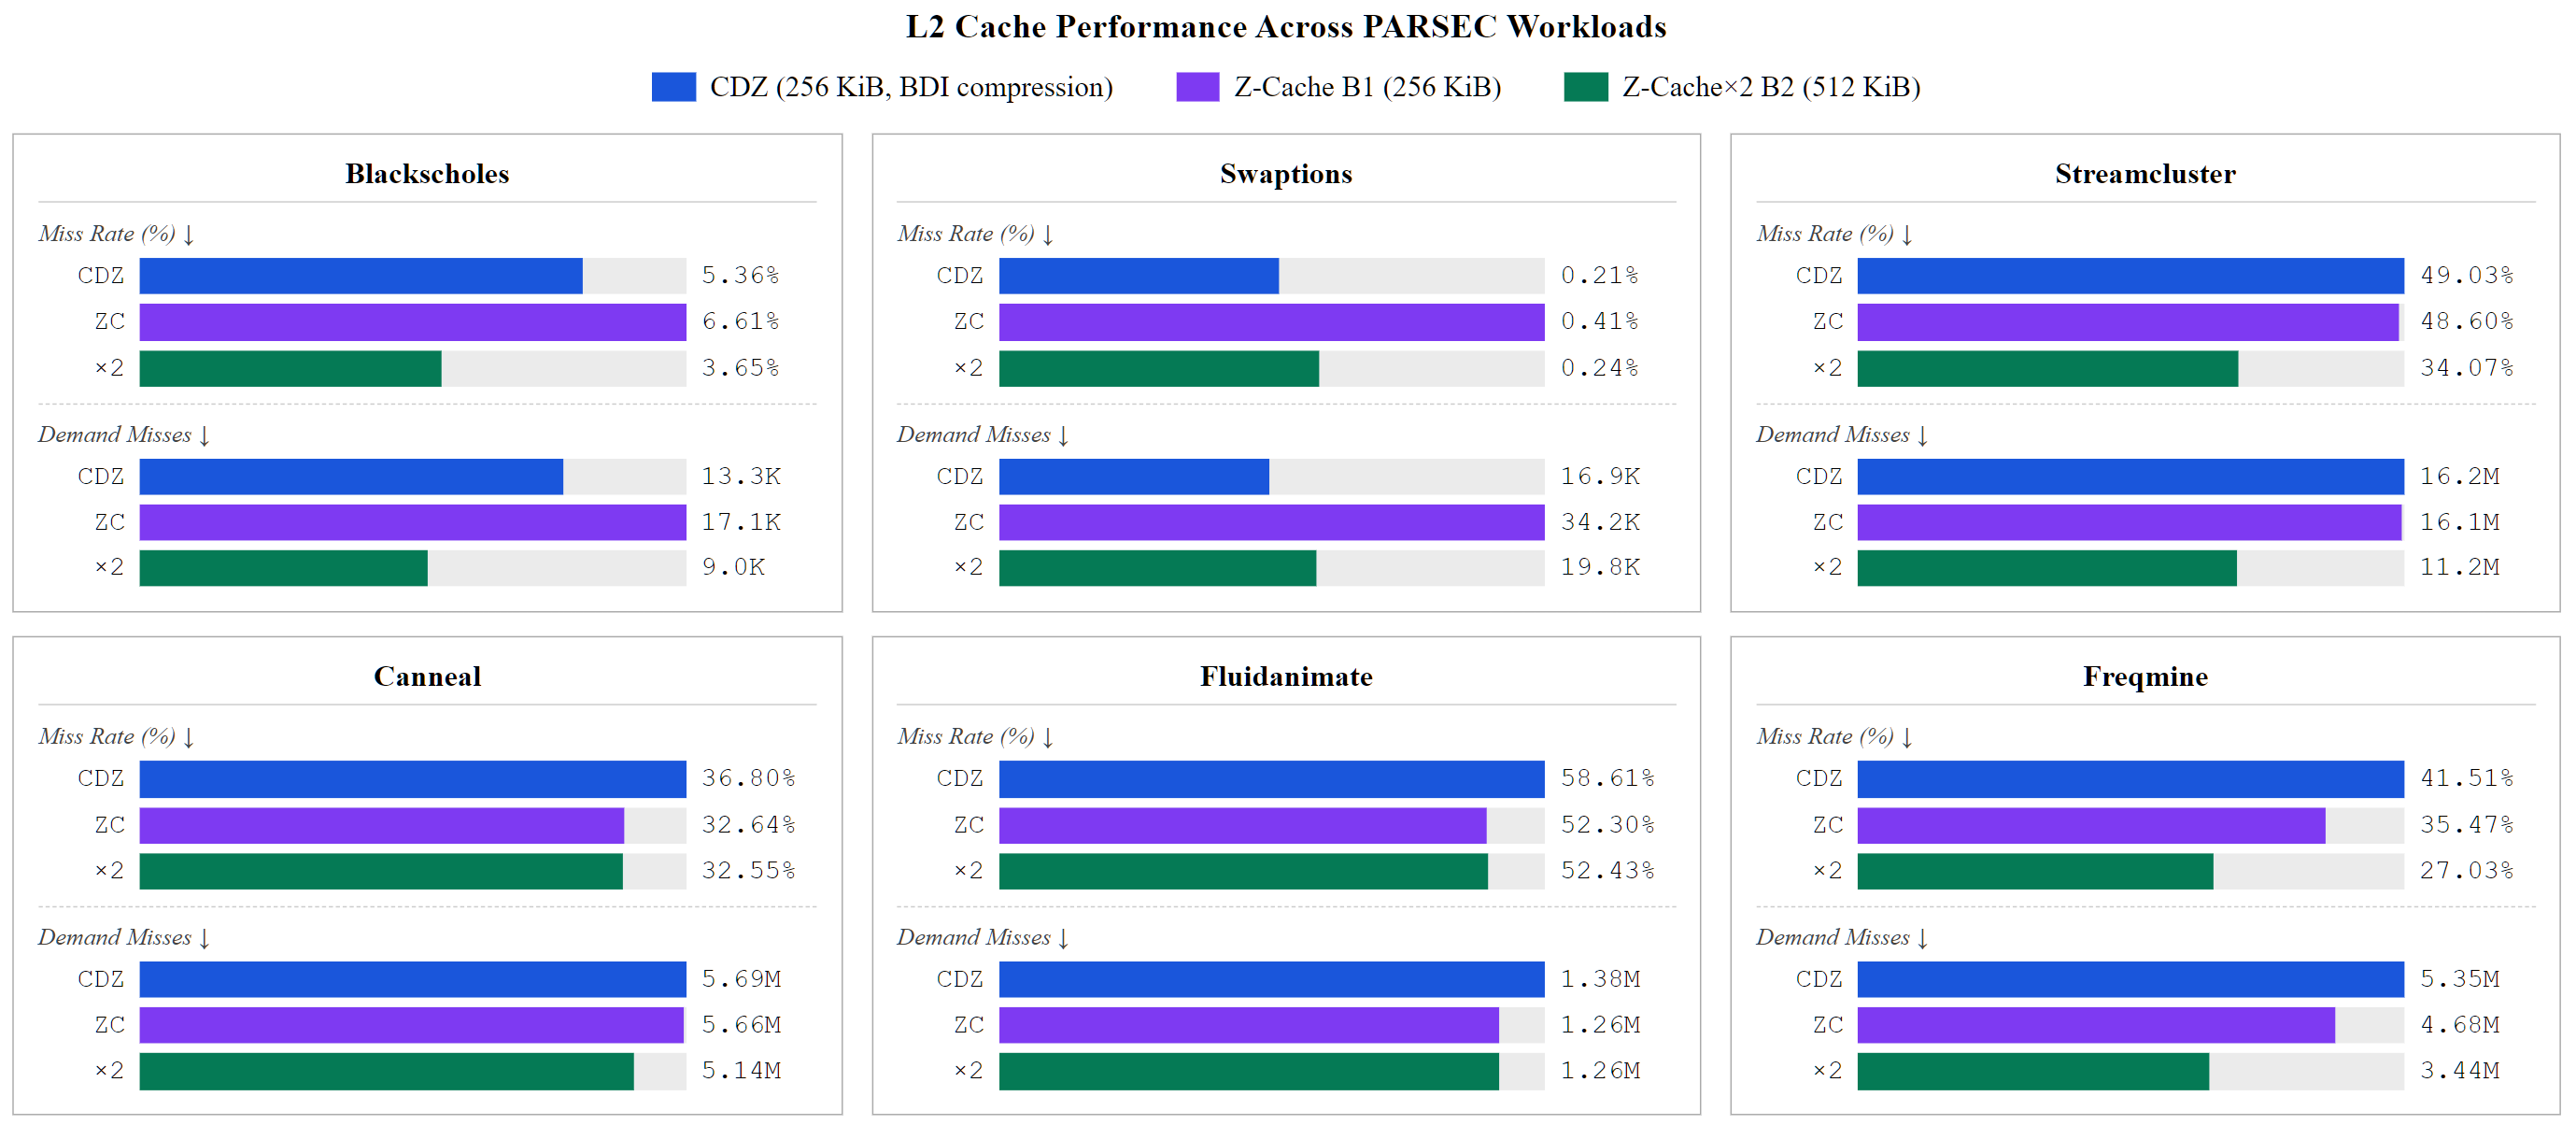
\includegraphics[width=\textwidth, keepaspectratio]{cdz-results.png}
  \caption{L2 miss rate (\%) and demand miss count for three cache
  configurations across six PARSEC workloads, simulated with gem5 full-system
  simulation (x86, 2-core, 16-way L2, 1\,THz simulated frequency).
  \textbf{CDZ}: Z-Cache (256\,KiB) augmented with BPC compression.
  \textbf{Z-Cache B1}: Z-Cache baseline (256\,KiB).
  \textbf{Z-Cache$\times$2 B2}: Z-Cache (512\,KiB). Bar widths are normalized
  to the worst-performing configuration per metric per workload. Area overhead:
  CDZ $\approx 1.15\times$, Z-Cache B1 $= 1.00\times$ (reference),
  Z-Cache$\times$2 B2 $\approx 1.90\times$. K $=$ thousands; M $=$ millions.}
  \label{fig:results}
\end{figure*}

\section{Conclusion and Future Work}
We presented CDZ-Cache, a decoupled unification of Z-Cache and BPC that
sidesteps the variable-block-size incompatibility through a buddy-allocated
data array fronted by fixed-size pointers. The design meets its goal of
requiring minimal changes to the underlying Z-Cache and BPC components, and on
compressible (financial) workloads it approaches the performance of a
Z-Cache twice its size; on workloads with poor intra-line similarity it
underperforms the baseline.

First and foremost, BPC is not an all-around high-performing compression
algorithm; it was chosen for its simplicity and ease of implementation. BPC
struggles with float compression, and completely fails when the data within a
cache line has low self-similarity, such as during graph exploration on large
graphs. A major point of future work is to choose a compression algorithm with
far better characteristics. CDZ-Cache's effectiveness with \textit{Swaptions}
shows that when the compression algorithm aligns with the nature of the data,
we can approach the performance of a simple Z-Cache twice as large.

The decoupled nature of the system might allow for multiple compression
algorithms that feed into the same data allocation system, with the smallest
block chosen for storage, and only a few additional bits per allocation to
store the compression type. Compression logic generally consumes less die space
than SRAM, and a convergence point where performance expected for a cache twice
as large, for general-purpose CPU applications, in a die space half as large,
may be possible.

Additionally, our solution for defragmentation of the data array is by-and-large
a naive band-aid. The pseudo-random policy was chosen for its simplicity rather
than any theory of effectiveness, and relies on the fact that a buddy
allocator, that only has to shuffle 4 sizes all powers of two, has a very low
chance of external fragmentation. Our solution was mainly to avoid corner-case
errors rather than be any permanent solution. A much more intelligent approach
to defragmentation would be future work.

Finally, we had planned a system for ``sticky'' cache lines/segments early in
our project, but abandoned it out of time constraints. For future work, our
design would involve an LRU counter modifier that uses the cache line's
compression level to nudge highly compressed lines closer to the future, making
them less likely to be chosen as a victim by the replacement policy. This would
not be ideal for every policy --- highly complex ones such as
Mockingjay~\cite{shah2022mockingjay} might lose performance --- but would
improve compression performance, and would likely work fine with Z-Cache.

\section*{Acknowledgment}
The authors thank the ECE 757 instructional staff at UW--Madison.

\bibliographystyle{IEEEtran}
\bibliography{references}

\end{document}
